% ==============================================================================
%
% [ PROJ ] ASHE presentation
% [ FILE ] slides.tex
% [ AUTH ] Benjamin Skinner, Olivia Morales, William Doyle
% [ INIT ] 31 October 2022
%
% ==============================================================================

% --------------------------------------
% document settings
% --------------------------------------

% document class
\documentclass[aspectratio=169, t, 10pt]{beamer}

% packages
\usepackage[utf8]{inputenc}
\usepackage{fontspec}
\usepackage{datetime}
\usepackage{tikz}
\usepackage{forest}
\usepackage{tabularx}
\usepackage{booktabs}
\usepackage{caption}
\usepackage{graphicx}
\usepackage[natbibapa]{apacite}
\usepackage{url}
\usepackage{amstext}
\usepackage[justification=raggedright]{caption}
\usepackage[flushleft]{threeparttable}
\usepackage{pgf}
\usepackage{mathtools}
\usepackage{multicol}
\usepackage{xcolor}
\usepackage[fixed]{fontawesome5}
\usepackage[first=1, last=100]{lcg}
\usepackage{xifthen}
\usepackage{ulem}
\usepackage{longtable}
\usepackage{multicol}

% tikz settings
\usetikzlibrary{positioning,
  shapes.multipart,
  calc,
  decorations.pathreplacing,
  decorations.text,
  calligraphy,
  arrows}

% --------------------------------------
% external inputs
% --------------------------------------

% ==============================================================================
%
% [ PROJ ] ASHE presentation
% [ FILE ] beamer_settings.tex
% [ AUTH ] Benjamin Skinner, Olivia Morales, William Doyle
% [ INIT ] 31 October 2022
%
% ==============================================================================

% --------------------------------------
% personalization settings
% --------------------------------------

% general links
\newcommand{\twr}{https://twitter.com/}
\newcommand{\mt}{mailto:}
\newcommand{\web}{https://}
\newcommand{\git}{https://github.com/}

% links for BS
\newcommand{\bts}{btskinner.io}
\newcommand{\webbs}{\web\bts}
\newcommand{\twrbs}{btskinner}
\newcommand{\gitbs}{btskinner}
\newcommand{\mtbs}{btskinner@coe.ufl.edu}

% links for OM
\newcommand{\onm}{}
\newcommand{\webom}{}
\newcommand{\twrom}{olivianmo}
\newcommand{\gitom}{onmorales23}
\newcommand{\mtom}{oliviamorales@ufl.edu}

% links for WD
\newcommand{\wrd}{my.vanderbilt.edu/willdoyle}
\newcommand{\webwd}{\web\wrd}
\newcommand{\twrwd}{wdoyle42}
\newcommand{\gitwd}{wdoyle42}
\newcommand{\mtwd}{w.doyle@vanderbilt.edu}

% replication code link
% \newcommand{\gitrep}{btskinner/holc\_bb\_rep}

% directories
\newcommand{\figdir}{../figures}
\newcommand{\tabdir}{../tables}
\newcommand{\imgdir}{../img}
\newcommand{\bibdir}{../bib}

% logos
\newcommand{\brlogo}{\imgdir/UF_Monogram.eps}
\newcommand{\primarylogo}{\imgdir/College-of-Education-UF.eps}

% --------------------------------------
% math macros
% --------------------------------------

\newcommand{\bbeta}{\boldsymbol{\beta}}
\newcommand{\bgamma}{\boldsymbol{\gamma}}
\newcommand{\bBeta}{\boldsymbol{B}}
\newcommand{\balpha}{\boldsymbol{\alpha}}
\newcommand{\bdelta}{\boldsymbol{\delta}}
\newcommand{\boldeta}{\boldsymbol{\eta}}
\newcommand{\btheta}{\boldsymbol{\theta}}
\newcommand{\bpsi}{\boldsymbol{\psi}}
\newcommand{\bphi}{\boldsymbol{\phi}}
\newcommand{\bc}{\mathbf{c}}
\newcommand{\bw}{\mathbf{w}}
\newcommand{\bx}{\mathbf{x}}
\newcommand{\by}{\mathbf{y}}
\newcommand{\bz}{\mathbf{z}}
\newcommand{\bW}{\mathbf{W}}
\newcommand{\bX}{\mathbf{X}}
\newcommand{\bY}{\mathbf{Y}}
\newcommand{\bZ}{\mathbf{Z}}


% --------------------------------------
% programming macros
% --------------------------------------

\newcommand{\itemcolor}[1]{
    \renewcommand{\makelabel}[1]{\color{#1}\hfil ##1}
}

% document background
\newcommand{\bg}[1]{
  \setbeamertemplate{background canvas}
  {\makebox[\paperwidth][c]{\begin{tikzpicture}
      \node[opacity=.22]{
        \includegraphics[width=\paperwidth]{\imgdir/#1}};
    \end{tikzpicture}}}
}

% --------------------------------------
% formatting macros
% --------------------------------------

% spacing
\newcommand{\hs}{\hspace{.25em}}

% color macros
\definecolor{black}{RGB}{0,0,0} % none more black (Pantone Black C)
\definecolor{white}{RGB}{255,255,255} % none more white
\definecolor{uf_blue}{RGB}{0,33,165} % UF blue (PMS 287; #0021A5)
\definecolor{uf_orange}{RGB}{250,70,22} % UF orange (PMS 172; #FA4616)
\definecolor{uf_blue_m}{RGB}{108,154,195} % muted UF blue (PMS 216-5; #6C9AC3)
\definecolor{uf_orange_m}{RGB}{226,143,65} % muted UF orange (PMS 46-3; #E28F41)
\definecolor{uf_green}{RGB}{94,142,63} % UF green (PMS 293-2; #5E8E3F)
\definecolor{uf_yellow}{RGB}{252,175,23} % muted UF orange (PMS 18-1; #FCAF17)
\definecolor{tw_blue}{RGB}{29,161,242} % twitter blue (#1DA1F2)

% set colors
\setbeamercolor{title}{fg = black}
\setbeamercolor{frametitle}{fg = black}
\setbeamercolor{framesubtitle}{fg = black}
\setbeamercolor{normal text}{fg = black}
\setbeamercolor{description item}{fg = uf_orange}
\setbeamercolor{block title}{fg = black}
\setbeamercolor{button}{bg = uf_blue}
\setbeamercolor{enumerate item}{fg = uf_blue}
\setbeamertemplate{itemize item}{\color{uf_yellow}$\blacktriangleright$}
\setbeamertemplate{itemize subitem}{\footnotesize\color{uf_yellow}$\blacktriangleright$}
\setbeamertemplate{itemize/enumerate subbody begin}{\footnotesize}
\setbeamercolor{math text}{fg=white}

% headers
\setbeamerfont{framesubtitle}{series = \itshape}

% fonts 
\setmainfont{Avenir Light} 
\setsansfont{Avenir Light} 
\setmonofont{Menlo}

% beamer theme and options
\usetheme{default}
\beamertemplatenavigationsymbolsempty
\setbeamercovered{transparent}
% \addtobeamertemplate{frametitle}{}{\vspace{-1.5em}}
% \addtobeamertemplate{framesubtitle}{}{\vspace{-1em}}
% \setbeamertemplate{caption}{\raggedright\insertcaption\par}

% add lower right logo; twitter handles
\addtobeamertemplate{frametitle}{}{%
  \vspace*{-0.5em}
  \begin{tikzpicture}[remember picture, overlay]
    \node[anchor=south east, xshift = -.2em, yshift = .2em]
    at (current page.south east)
    {\includegraphics[height=.9em]{\brlogo}};
    \node[anchor=south west, xshift = .2em, yshift = .2em]
    at (current page.south west)
    {\href{\twr\twrbs}{\footnotesize\textcolor{tw_blue}{\faTwitter}\twrbs}
    \href{\twr\twrom}{\footnotesize\textcolor{tw_blue}{\faTwitter}\twrom}
    \href{\twr\twrwd}{\footnotesize\textcolor{tw_blue}{\faTwitter}\twrwd}};
  \end{tikzpicture}
}

% make bibliography smaller
\renewcommand*{\bibfont}{\scriptsize}

% make citations smaller
\makeatletter
\DeclareRobustCommand\citep
{\begingroup\scriptsize\NAT@swatrue\let\NAT@ctype\z@\NAT@partrue
  \@ifstar{\NAT@fulltrue\NAT@citetp}{\NAT@fullfalse\NAT@citetp}}
\makeatother

% table alignment
\newcommand{\RR}{\raggedright\arraybackslash}
\newcommand{\RL}{\raggedleft\arraybackslash}


% --------------------------------------
% repeated text
% --------------------------------------

\newcommand{\fignote}[1]{\caption*{\tiny {\bfseries Note.} #1}}

% --------------------------------------
% begin document
% --------------------------------------

\begin{document}

% ~~~~~~~~~~~~~~~~~~~~~~~~~~~~~~~~~~~~~~~~~~~~~~~~~~~~~~~~~~~~~~~~~~~~~~~~~~~~~~
% title slide
% ~~~~~~~~~~~~~~~~~~~~~~~~~~~~~~~~~~~~~~~~~~~~~~~~~~~~~~~~~~~~~~~~~~~~~~~~~~~~~~

\title{\LARGE Employing Machine-Learning Approaches \\ to Predict Incomes 
of Recent College Graduates} 
\date{16 November 2022 \\
Association for the Study of Higher Education Annual Conference | Las Vegas, NV}
\author{%
  \begin{tabular}{ccc}
    {\Large Benjamin T. Skinner}
    & {\Large Olivia Morales}
    & {\Large William R. Doyle} \\
    University of Florida & University of Florida & Vanderbilt University \\
    \href{\twr\twrbs}{\textcolor{tw_blue}{\faTwitter}\hs\twrbs} &
    \href{\twr\twrom}{\textcolor{tw_blue}{\faTwitter}\hs\twrom} &
    \href{\twr\twrwd}{\textcolor{tw_blue}{\faTwitter}\hs\twrwd}  & \\
  \end{tabular}
}

\institute{\includegraphics[width = .5\textwidth]{\primarylogo}}

{
  \bg{uf_coe_1}
  \begin{frame}
    \titlepage
  \end{frame}
}

% ~~~~~~~~~~~~~~~~~~~~~~~~~~~~~~~~~~~~~~~~~~~~~~~~~~~~~~~~~~~~~~~~~~~~~~~~~~~~~~
% SLIDES
% ~~~~~~~~~~~~~~~~~~~~~~~~~~~~~~~~~~~~~~~~~~~~~~~~~~~~~~~~~~~~~~~~~~~~~~~~~~~~~~

% Introduction
\begin{frame}
  \frametitle{The Prediction Business for Returns to Higher Education}
  \begin{block}{What we know}
    \begin{itemize}
    	\item Wealth of scholarship to support economic returns from
          higher education
          \citep{card:1995, Card:1999, Card:2001, doyle2016educearn, Oreopoulous_Petronijevic_2013}
    	\item Prior analyses limited by access to institution-level data not widely available 
   	 \begin{itemize}
    		\item The publication of the College Scorecard (2015) changed the higher education \\
		research landscape, with national institutional-level
                data now publicly accessible
                \citep{obama_2013}
   	 \end{itemize}
    \end{itemize}
  \end{block}
  \begin{block}{Examining existing research}
    \begin{itemize}
    \item Standard econometric approaches to estimating earnings \\
    are vulnerable to researcher bias and produce less accurate predictions
    \item Machine learning methods provide a more useful alternative (predictions \\
    made algorithmically, based on features of the data)
    \end{itemize}
  \end{block}
\end{frame}

% Our focus/guiding questions
\begin{frame}
  \frametitle{Our focus \& guiding research questions}
  \begin{block}{Project focus}
    \centering
    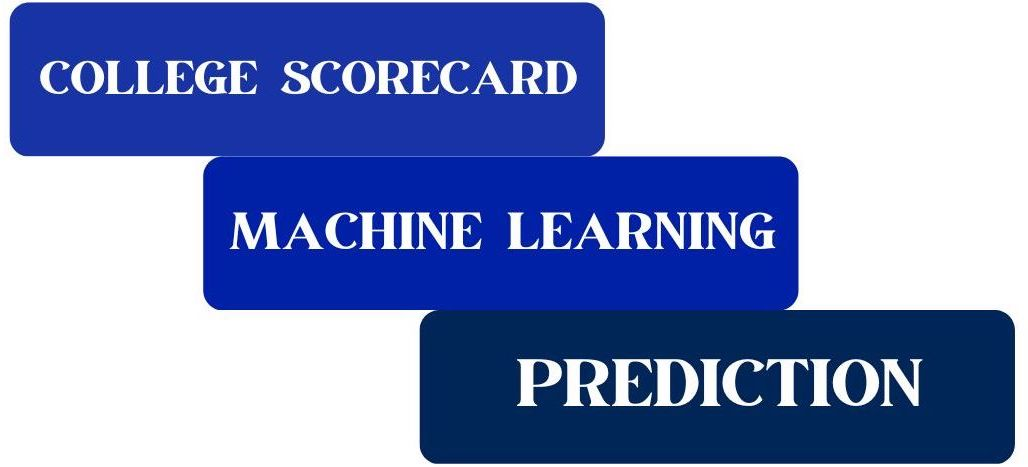
\includegraphics[scale = 0.2]{\imgdir/project_flow.jpg}
  \end{block}
  \begin{block}{Research questions}
    \begin{enumerate}
        \item What institutional\slash program level variables are most
          predictive of median first-year earnings?
        \item What are the patterns of association (positive\slash negative)
          for these variables?
    \end{enumerate}
   \end{block}
\end{frame}

% Data
\begin{frame}
  \frametitle{Data}
    \begin{block}{College Scorecard}
      \begin{itemize}
      \item 2019-2020 
      \item Includes over 2,000 variables for 6,700 accredited higher
        education institutions (HEIs) in the U.S.
      \item Significant portions of the data are privacy suppressed
      \end{itemize}
    \end{block}
  \begin{block}{American Community Survey (ACS)}
    \begin{itemize}
    \item 2015-2019
    \item Geography of interest: County level (using FIPS)
    \item Matching HEIs with unique county FIPS codes
    \item Helps recover information lost from missing data in the Scorecard
    \end{itemize}
  \end{block}
\end{frame}

% Tidymodels explanation
\begin{frame}
  \frametitle{Data preprocessing and model building with Tidymodels}
  \begin{block}{Tidymodels as a framework}
    \begin{itemize}
    \item Proposed by \citet{Kuhn_Silge_2022}, Tidymodels provides a
      succinct framework for preprocessing data to eventually use in
      fitting successive models and delineating overall workflow
     \end{itemize}
   \end{block}
   \begin{block}{}
     \vspace{-.75cm}%adapt
     \centering
        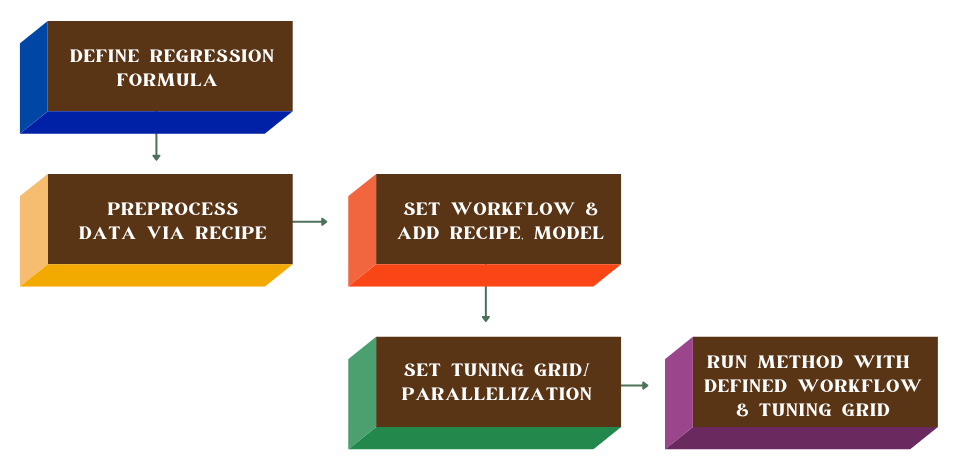
\includegraphics[scale = 0.4]{\imgdir/tidymodels_example.png}
   \end{block}   
\end{frame}

% Methodology
\begin{frame}
  \frametitle{Prediction via regression-based machine learning methods}
  \begin{block}{Elastic net regularization}
    \begin{itemize}
    \item Combines LASSO/ridge regression penalties to mitigate issues
      of bias and variance introduction in your statistical model
    \item Helpful in producing more parsimonious models (removes
      irrelevant predictors)
    \end{itemize}
  \end{block}
  \begin{block}{Random forests}
    \begin{itemize}
      \item Ensemble machine learning method particularly popular in
        gauging variable importance in a regression model
      \item Randomly samples covariates in a regression model, splits
        observations on covariates to maximize reduction of RMSE 
      \item Model builds successive trees to eventually including all
        covariates in the model, averaging over all trees to determine
        variable importance (reduction in RMSE)
      \end{itemize}
   \end{block}
\end{frame}
      
      
% Random forest: A visualization
\begin{frame}
  \frametitle{Random forest: A visualization}\citep{koehrsen_2018}
    \centering
        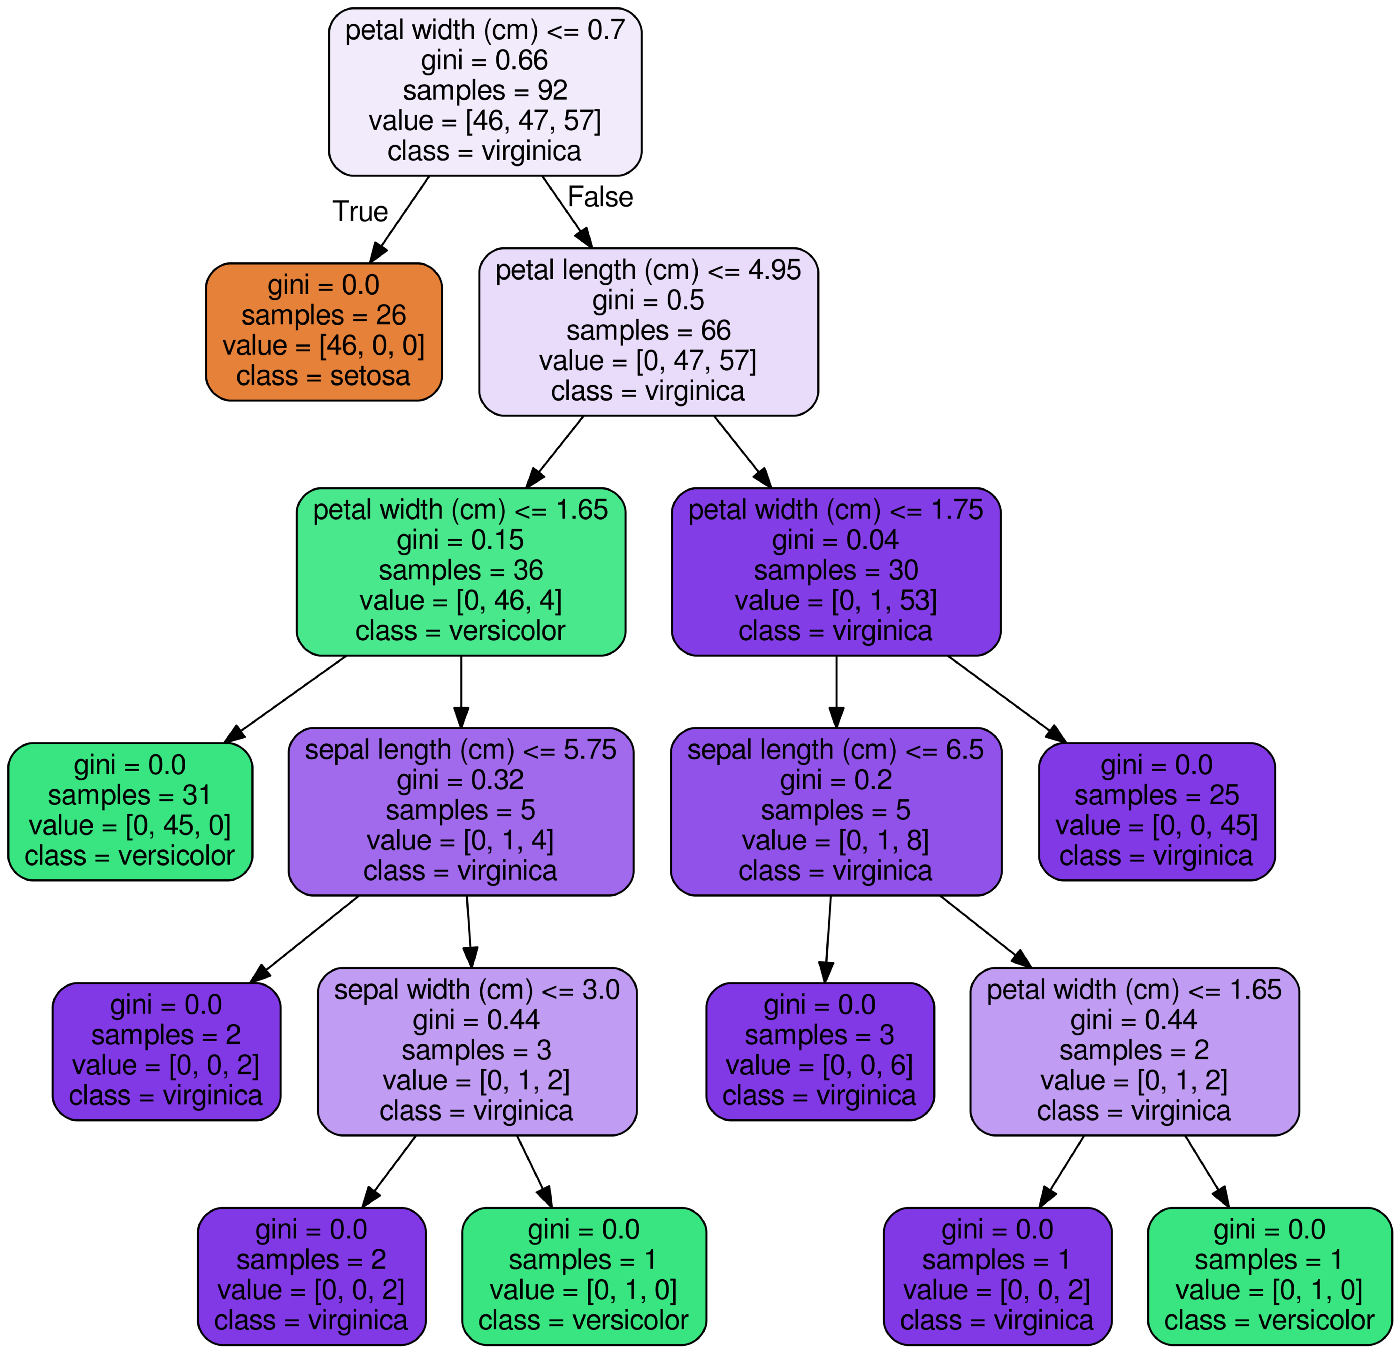
\includegraphics[width=.5\linewidth]{\imgdir/rf_viz.png}
 \end{frame}

% Findings I
\begin{frame}
  \frametitle{Elastic net regularization}
    \centering
        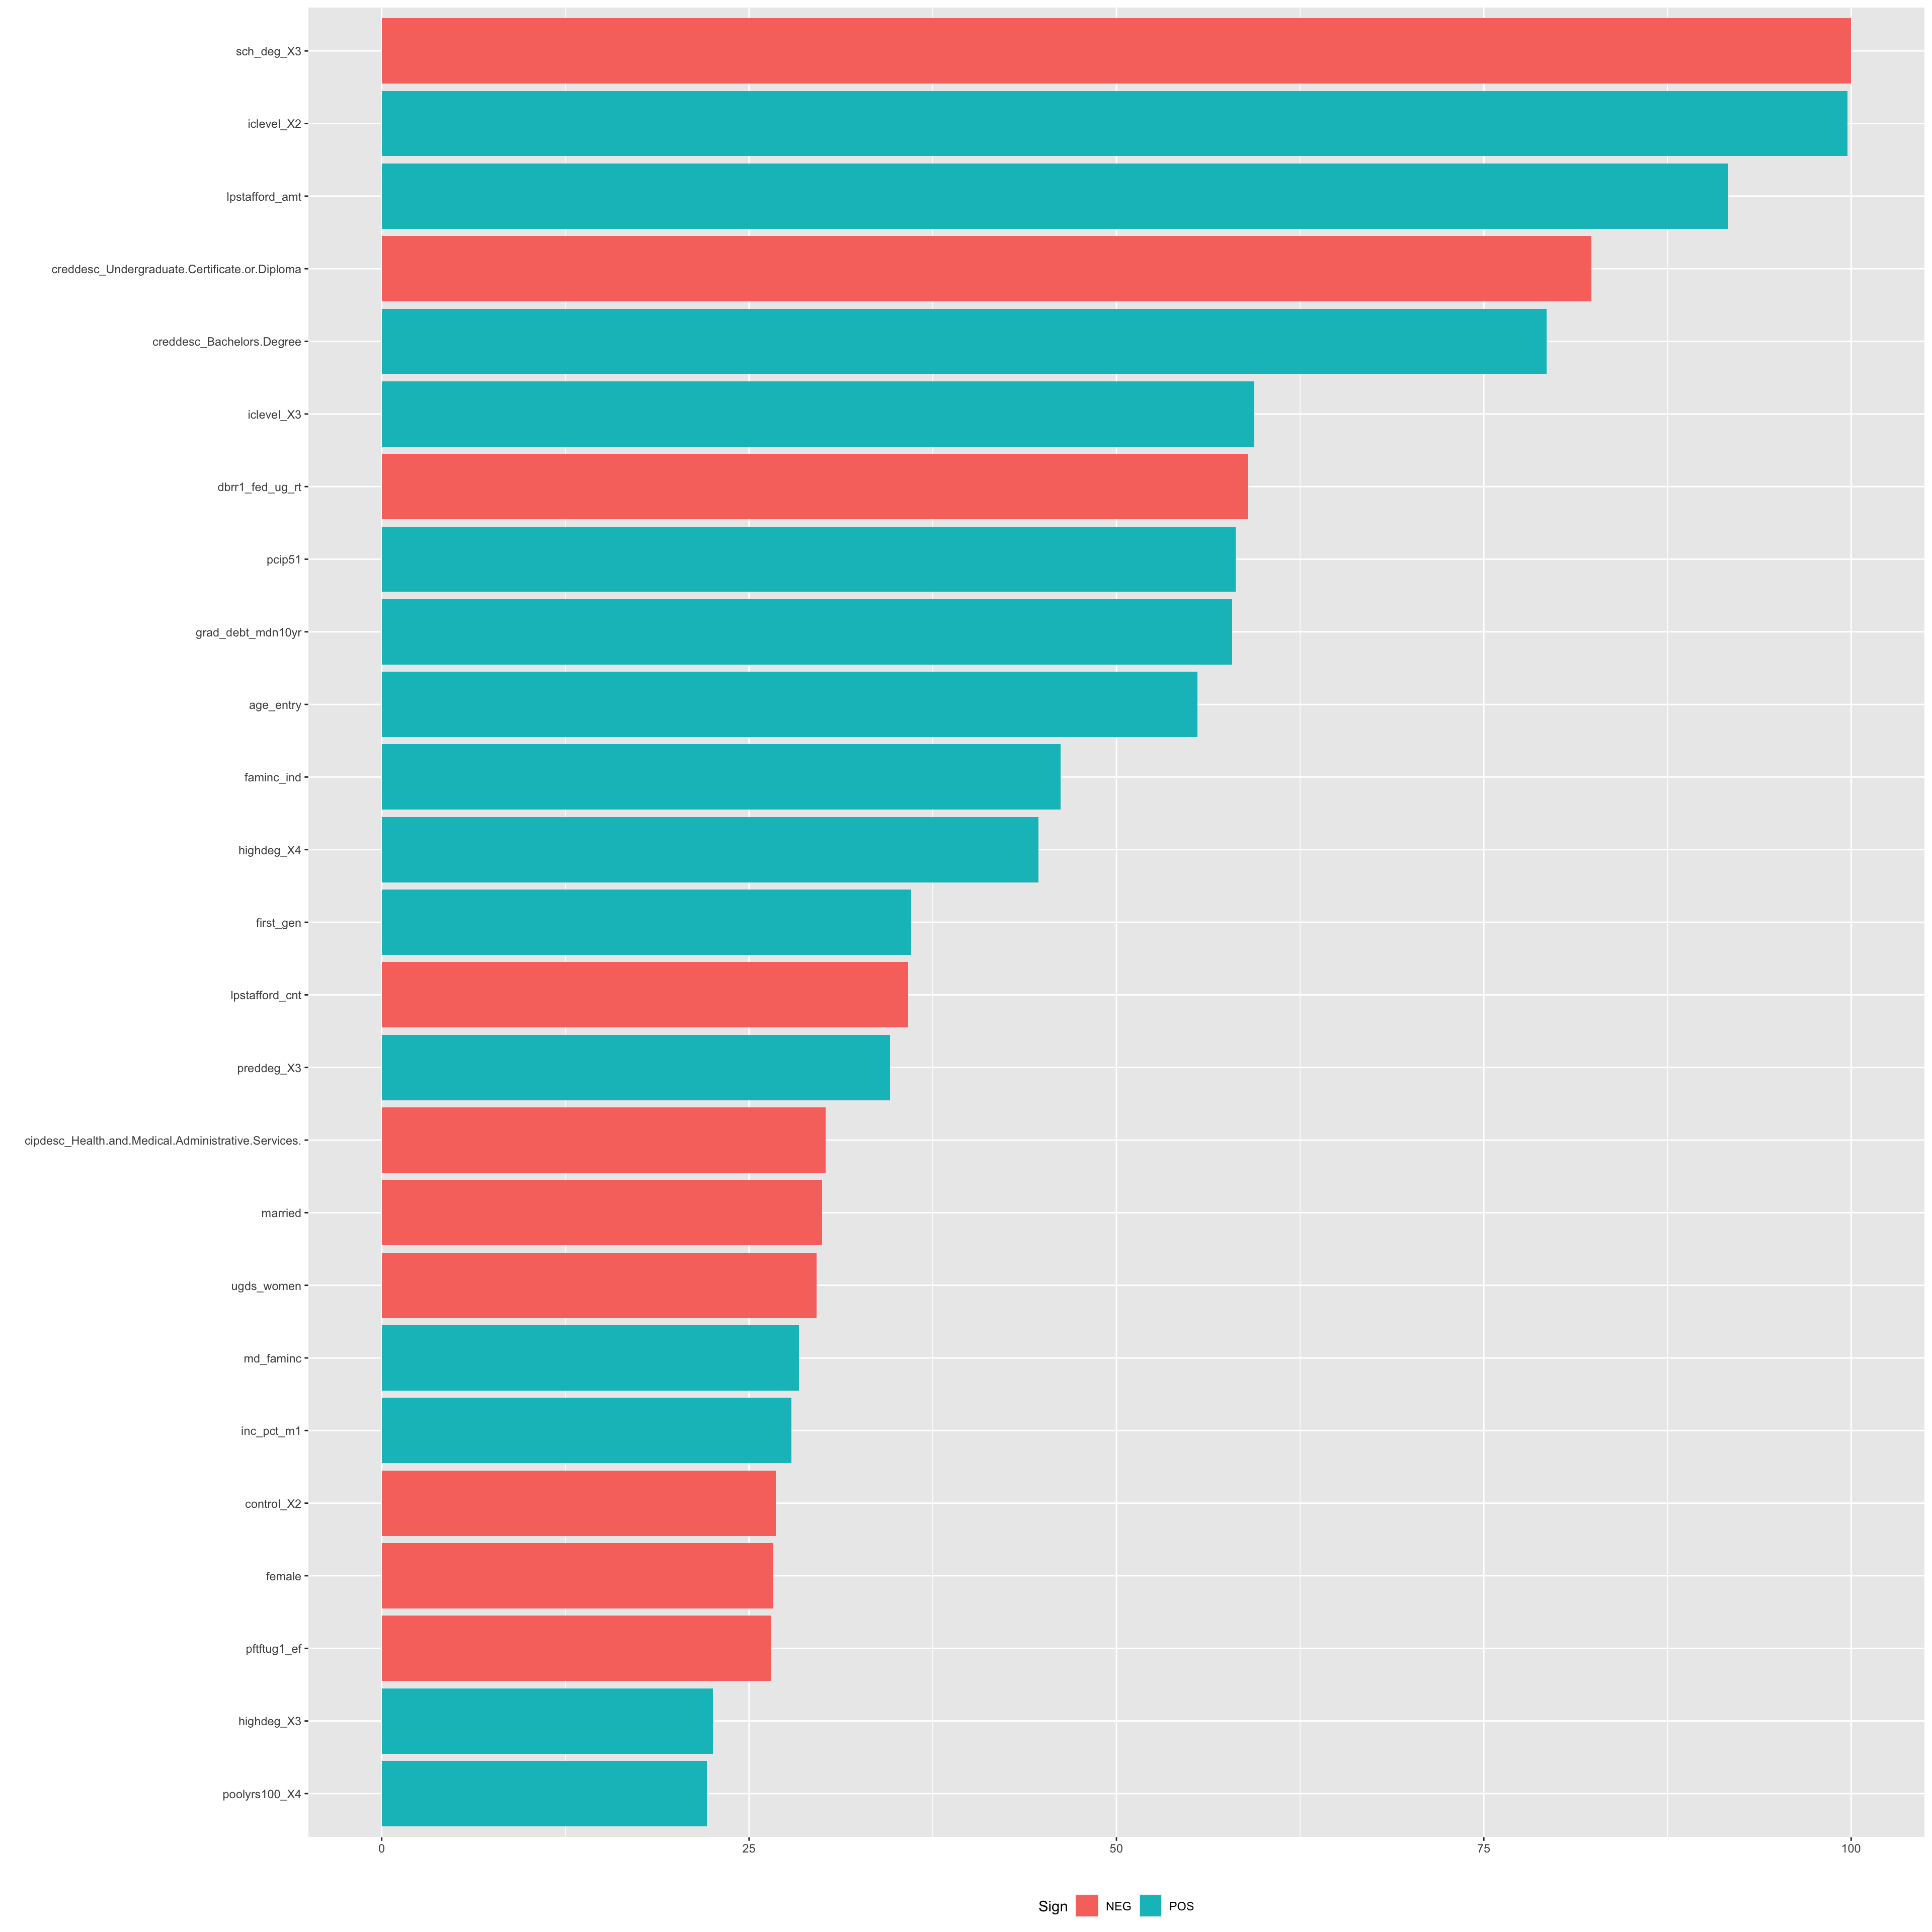
\includegraphics[width=.5\linewidth]{\imgdir/enet_fig.png}
 \end{frame}

% Findings II
\begin{frame}
  \frametitle{Random forest model: Variable importance}
    \centering
        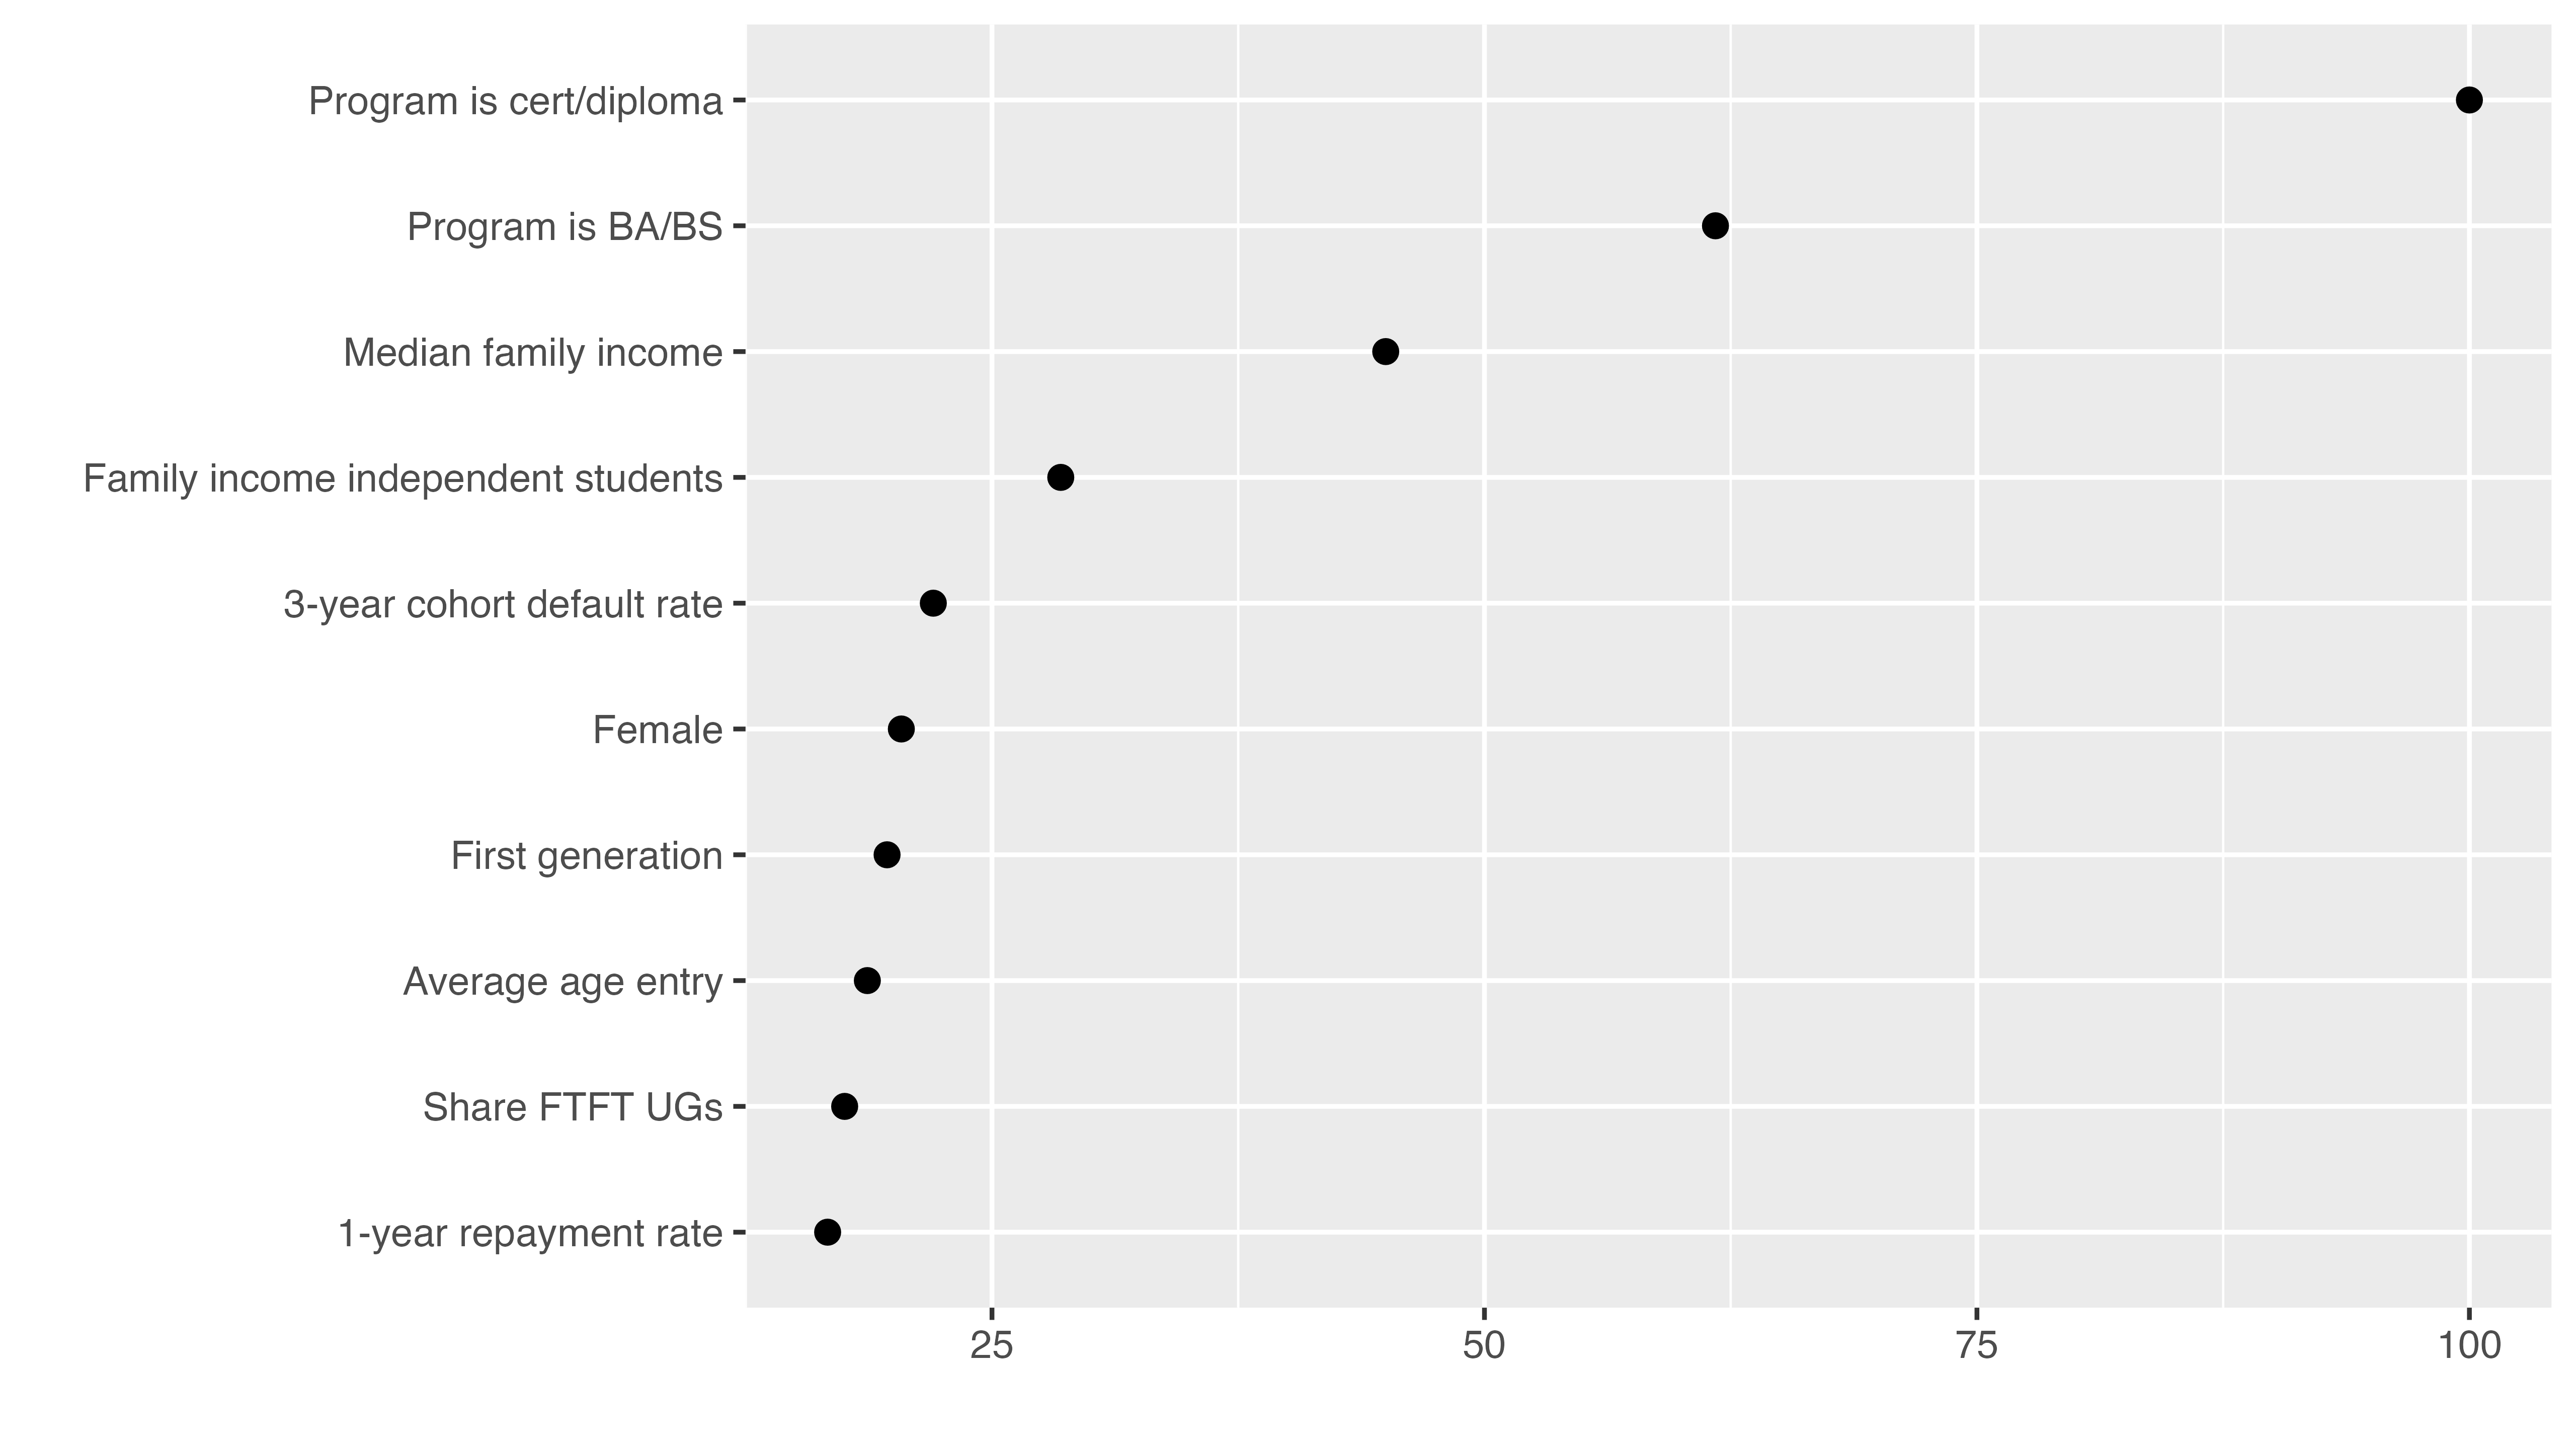
\includegraphics[scale = 0.35]{\imgdir/rf_vi.png}
 \end{frame}

% Takeaways/Conclusions
\begin{frame}
  \frametitle{Discussion\slash conclusion}
  \begin{block}{Elastic net model}
    \begin{itemize}
    \item Expected predictors 
      \begin{itemize}
         \item Predominant degree awarded, Bachelor's (positive)
         \item Level of institution, 4-year (positive)
      \end{itemize}
    \item Unexpected predictors
       \begin{itemize}
         \item Total outstanding federal direct loan balance (positive)
         \item Undergraduate federal student loan dollar-based 1-year
           repayment rate borrower count (negative)
      \end{itemize}    
    \end{itemize}
  \end{block}
  \begin{block}{Random forest model}
    \begin{itemize}
    \item Variable importance
      \begin{itemize}
        \item Level of credential (Undergraduate certificate or
          diploma /& Bachelor's degree)
        \item Median family income
        \item Average family income for independent students
       \end{itemize}
    \end{itemize}
   \end{block}    
\end{frame}
 
% ~~~~~~~~~~~~~~~~~~~~~~~~~~~~~~~~~~~~~~~~~~~~~~~~~~~~~~~~~~~~~~~~~~~~~~~~~~~~~~
% THANK YOU
% ~~~~~~~~~~~~~~~~~~~~~~~~~~~~~~~~~~~~~~~~~~~~~~~~~~~~~~~~~~~~~~~~~~~~~~~~~~~~~~

{
  \bg{uf_coe_6}
  \begin{frame}
    \begin{center}
      \huge
      \vfill
      Thank You! \\
      \vfill
      % \large
      % Replication files \\
      \small
      % \begin{tabular}{l}
      %   \href{\git\gitrep}{\faCode\hs\git\gitrep} \\
      % \end{tabular}
      % \vfill
      \begin{tabular}{lll}
        {\Large Olivia N. Morales}  \\
        \href{\mt\mtom}{\faEnvelope\hs\mtom}\\
        \href{\twr\twrom}{\faTwitter\hs\twrom} \\
        \href{\git\gitom}{\faGithub\hs\gitom} \\
      \end{tabular}
      \vfill
      \includegraphics[width=.5\linewidth]{\primarylogo}
      \vfill
    \end{center}
  \end{frame}
}

% ~~~~~~~~~~~~~~~~~~~~~~~~~~~~~~~~~~~~~~~~~~~~~~~~~~~~~~~~~~~~~~~~~~~~~~~~~~~~~~
% REFERENCES
% ~~~~~~~~~~~~~~~~~~~~~~~~~~~~~~~~~~~~~~~~~~~~~~~~~~~~~~~~~~~~~~~~~~~~~~~~~~~~~~

\begin{frame}[allowframebreaks]
\frametitle{References}
\bibliographystyle{apacite}
\bibliography{\bibdir/csc_research.bib}
\end{frame}

\end{document}

%%%%%%%%%%%%%%%%%%%%%%%%%%%%%%%%%%%%%%%%%%%%%%%%%%%%%%%%%%%%%%%%%%%%%%%%%%%%%%%%
% End document
%%%%%%%%%%%%%%%%%%%%%%%%%%%%%%%%%%%%%%%%%%%%%%%%%%%%%%%%%%%%%%%%%%%%%%%%%%%%%%%%

